

\section{Proposed Approach: LLM-as-a-Verifier}
\subsection{Motivation}
\begin{wrapfigure}{r}{0.36\textwidth}
    \centering
    \vspace{-33pt}
    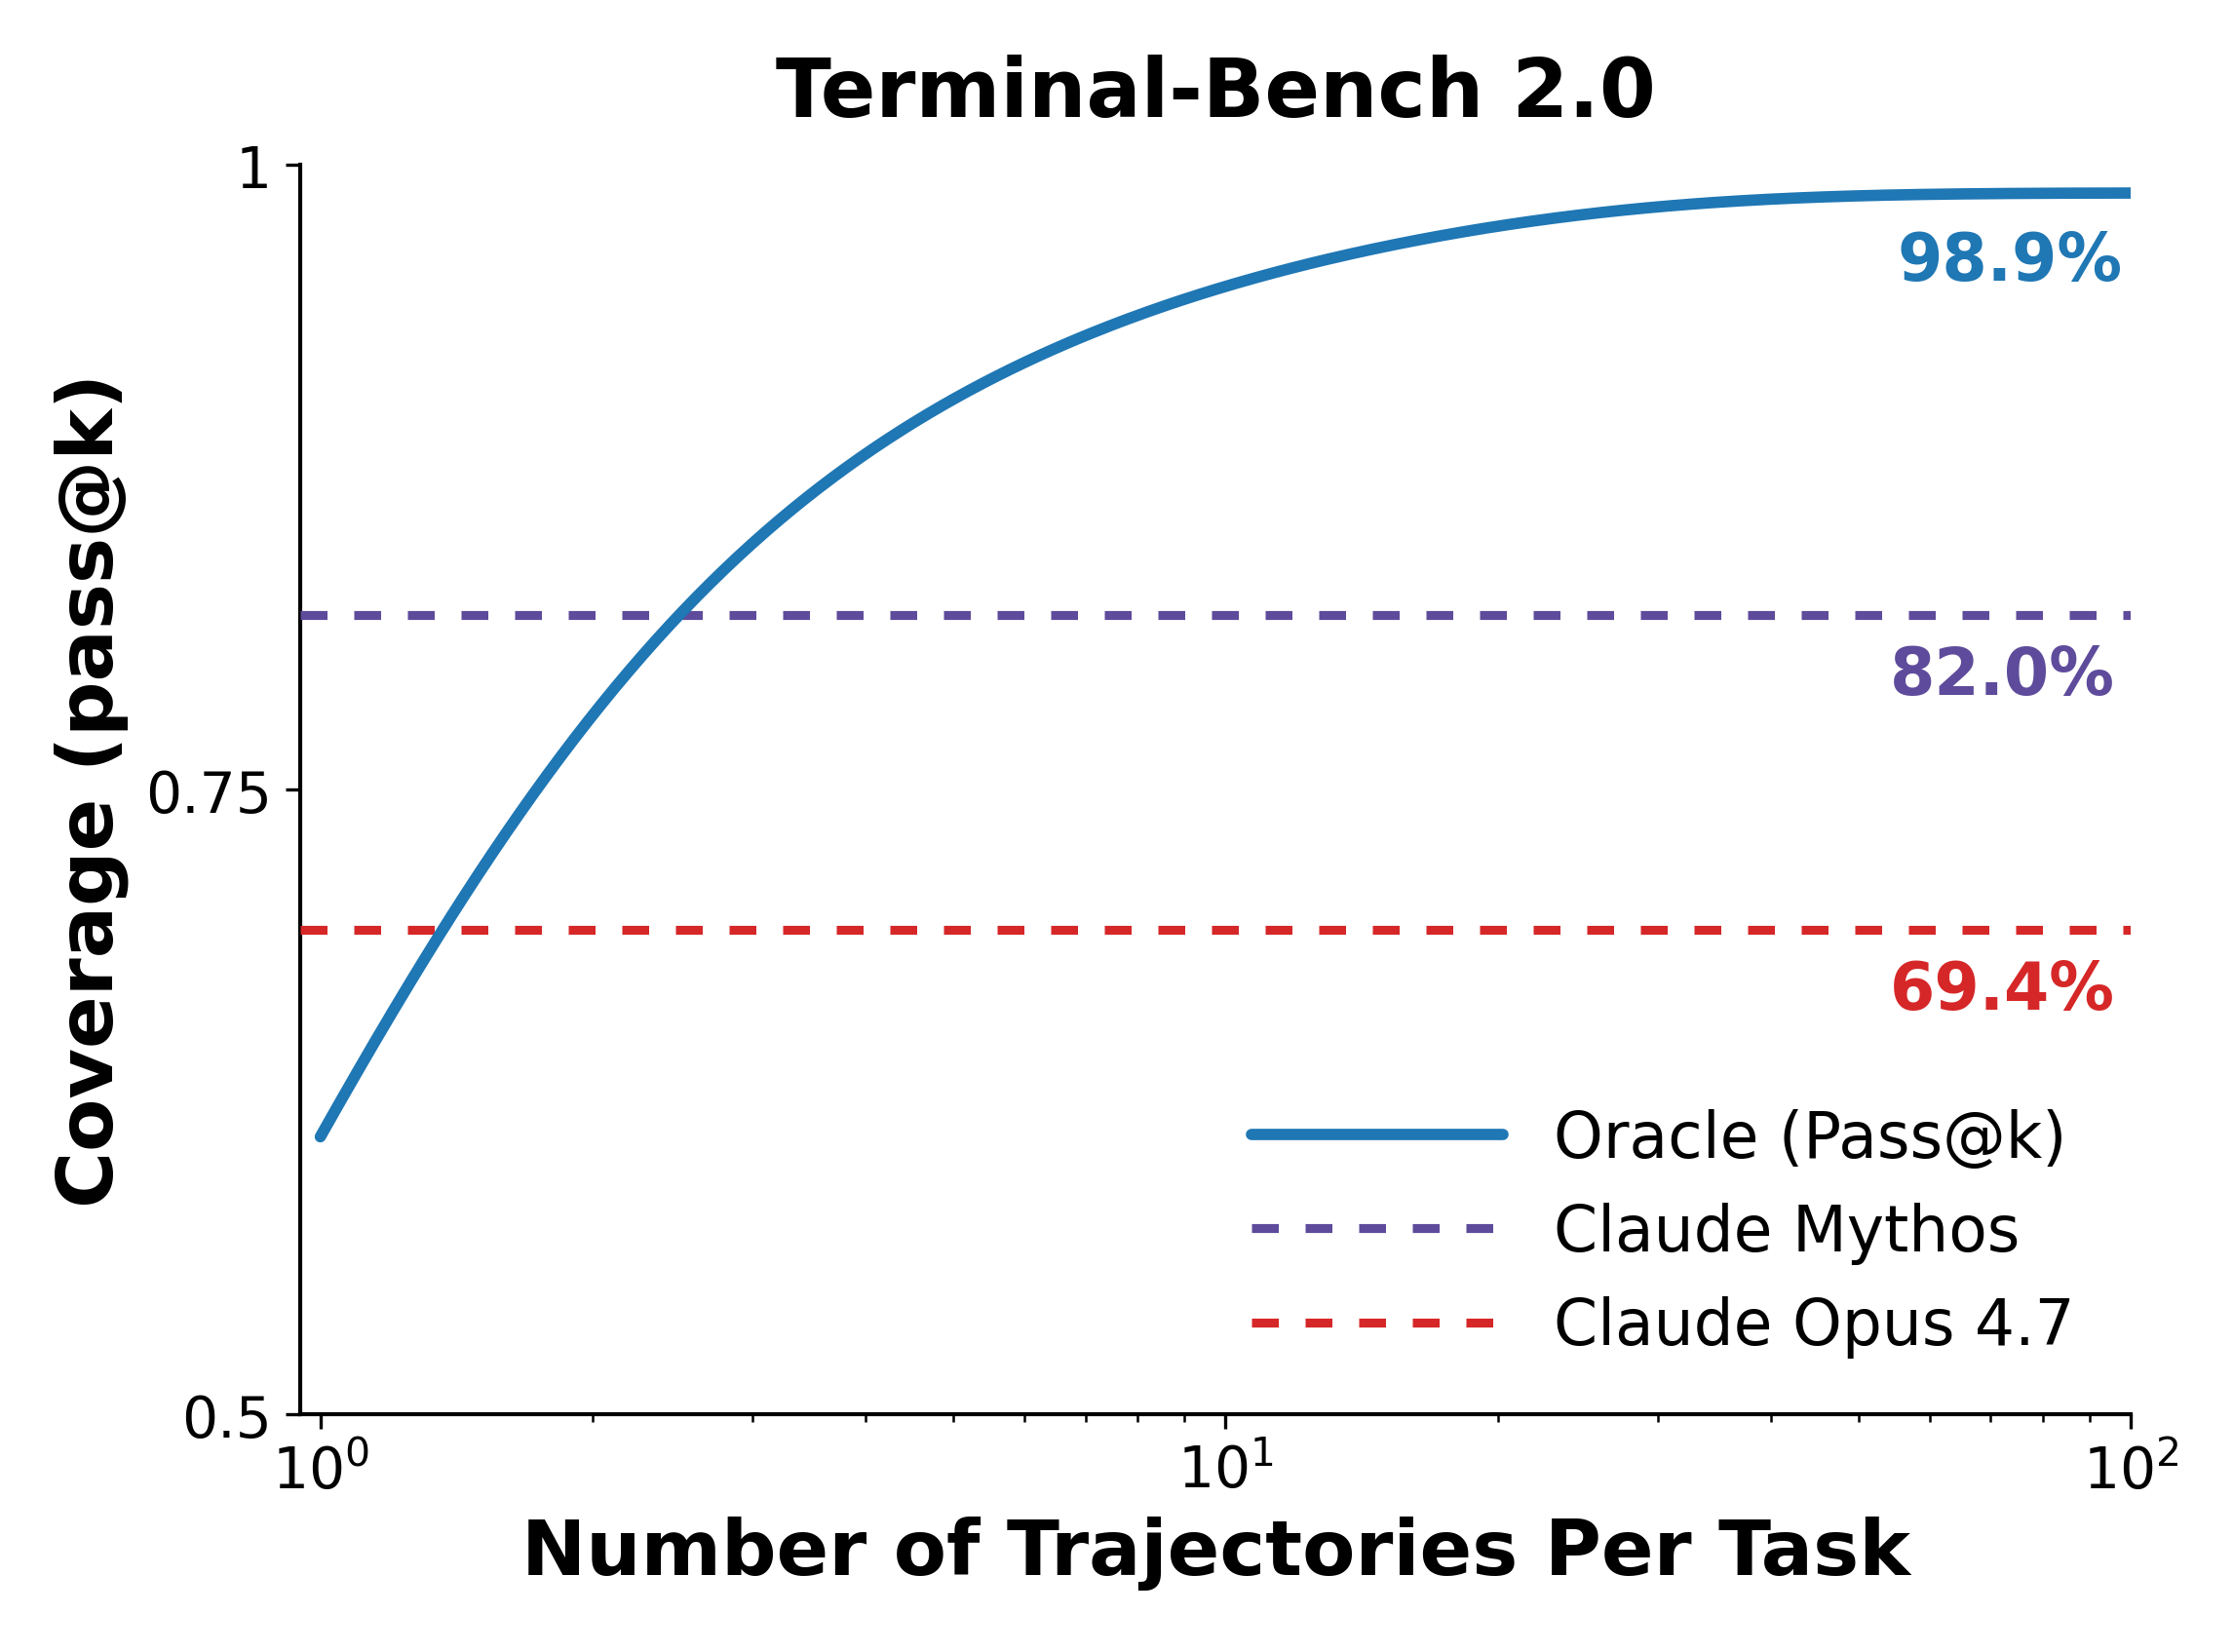
\includegraphics[width=\linewidth]{figures/oracle_bon_plot.png}
    \vspace{-16pt}
    \caption{Oracle Pass@$K$ reaches 98.9\% on Terminal-Bench~V2.}
    \label{fig:motivation}
    \vspace{-8pt}
\end{wrapfigure}
Most models already possess the capability to solve many tasks: when executed repeatedly, they often produce a correct solution at least once. As shown in Fig.~\ref{fig:motivation} (left), the fraction of solved tasks increases consistently as we scale the number of sampled trajectories on Terminal-Bench, assuming access to an oracle verifier that always picks the optimal trajectory. Under this setting, the success rate reaches 98.9\% when pooling trajectories across the full Terminal-Bench~V2 leaderboard, effectively solving nearly the entire benchmark. However, capturing this headroom requires a verifier that can reliably distinguish correct trajectories from incorrect ones. While standard LM judges~\citep{zheng_judging_nodate} can be used as verifiers, they fail to provide sufficiently fine-grained feedback. Specifically, they prompt the model to output a discrete score token and select the highest-probability token as the final score, collapsing the full scoring distribution into a single value. This leads to inherently coarse evaluations. When comparing complex solutions, standard LM judges often assign the same score, resulting in ties and failing to discriminate between them. As a result, coarse scoring induces a high tie rate (27\%) on Terminal-Bench, with distinct trajectories often collapsing to the same score, as illustrated in Figure~\ref{fig:judge_verifier}. One could instead train a reward model~\citep{stiennon_learning_2022}, but such methods are constrained by their training data and often fail to generalize across domains. These limitations motivate the need for a generalizable framework that can provide fine-grained verification signals.

\subsection{Methodology}
\textbf{Fine-Grained Reward Estimation.} By definition, a judge is one who forms an overall opinion and assigns a decision, whereas a verifier is one who confirms the truth or correctness of something and requires more detailed evaluations. To this end, we introduce LLM-as-a-Verifier, a probabilistic verification framework that provides fine-grained feedback by scaling scoring granularity, repeated evaluation, and criteria decomposition. 

Let $V_{\text{score}} = \{v_1, \ldots, v_G\}$ denote an ordered set of tokens representing discrete score levels. Given a task prompt $x$, a language model $p_\theta$, a criterion $c$, and two candidate trajectories $\tau_i$ and $\tau_j$, we construct scoring prompts and obtain their conditional distributions $p_{\theta}(v \mid x,c,\tau_i)$ and $p_{\theta}(v \mid x, c, \tau_j)$ by extracting the logprobs from $<score_A>$ and $<score_B>$ tags using the following prompt:
\begin{quote}
\small
\ttfamily
You are an expert [domain] reviewer. You will see a task description and two trajectories.

Evaluation Criteria: [domain specific criteria]

Task: \{task prompt\} \\
Trajectory A: \{A\} Trajectory B: \{B\}

Carefully analyze each trajectory, then provide your final scores:
\begin{verbatim}
<score_A> INTEGER_1_TO_20 </score_A>
<score_B> INTEGER_1_TO_20 </score_B>
\end{verbatim}

Rating Rules: Rate correctness on a 1--20 scale based on evaluation criteria (1 = incorrect, 10 = borderline, 20 = correct)

Note: We use a letter-based scale instead of digits to enable logprob extraction for granularity scaling. 
\end{quote}

Rather than collapsing each distribution to a single discrete score, we approximate the reward of a trajectory as:
\begin{equation}
R(x, \tau)
= \frac{1}{CK} \sum_{c=1}^{C} \sum_{k=1}^{K}
\sum_{g=1}^{G} p_{\theta}(v_g \mid x, c, \tau)\,\phi(v_g)
\label{eq:main}
\end{equation}
where $C$ is the number of evaluation criteria, $K$ is the number of repeated verifications, $G$ is the number of score tokens (granularity level), $p_{\theta}(v_g \mid x, c, \tau)$ is the probability assigned by model $\theta$ to score token $v_g$, and $\phi(v_g)$ maps each score token to a scalar value. 


We first normalize $R(x,\tau)\in[0,1]$ by the linear map $R\mapsto(R-\phi_{\min})/(\phi_{\max}-\phi_{\min})$. Then, we convert these continuous rewards into a pairwise preference using the Bradley--Terry model, treating $R(x,\tau)$ as the latent strength of trajectory $\tau$:
\begin{equation}
P(\tau_i \succ \tau_j \mid x)
\;=\; \frac{1}{1+\exp\!\big(-(R(x,\tau_i)-R(x,\tau_j))\big)},
\label{eq:pref}
\end{equation}

\begin{figure}[t]
    \centering
    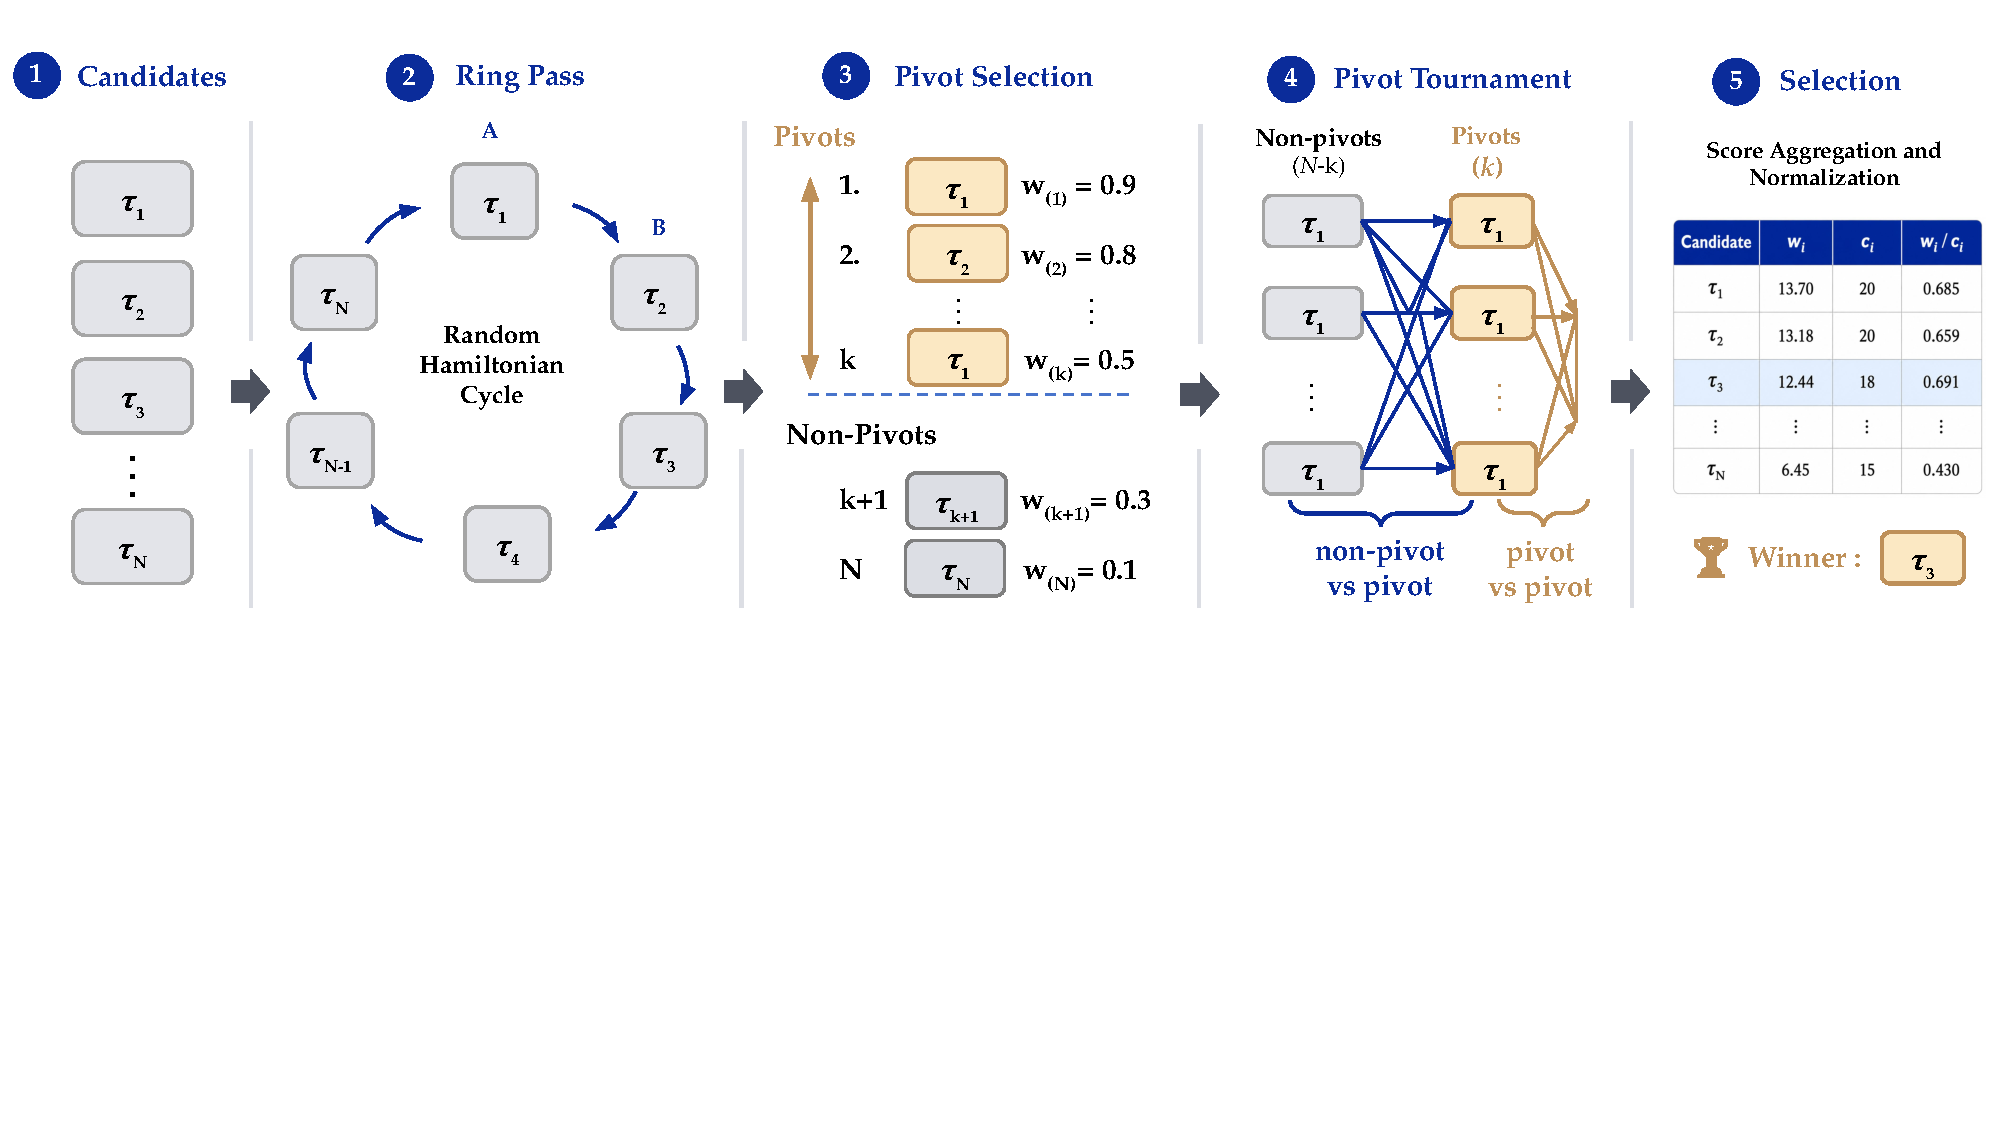
\includegraphics[width=\textwidth]{figures/pivot_tournament.pdf}
    \caption{\textbf{Probabilistic Pivot Tournament.} A five-stage pipeline for selecting the best of $N$ candidates under a constrained verification budget.
    \textbf{(1)~Candidates:} the pool $\{\tau_1,\dots,\tau_N\}$ to be ranked.
    \textbf{(2)~Ring pass:} a random Hamiltonian cycle scores the $N$ adjacent pairs so every candidate appears once in the ``A'' slot and once in ``B'', canceling the model's positional bias.
    \textbf{(3)~Pivot selection:} candidates are ranked by their ring-pass scores $w_{(i)}$, and the top-$k$ candidates form the pivot set $\mathcal{P}$.
    \textbf{(4)~Pivot tournament:} every \emph{non-pivot--vs--pivot} and \emph{pivot--vs--pivot} pair is scored via Eq.~\ref{eq:pref}, concentrating the budget on uncertain top candidates and cutting cost from $\mathcal{O}(N^2)$ to $\mathcal{O}(Nk)$.
    \textbf{(5)~Selection:} comparisons are aggregated into win mass $w_i$ and count $c_i$, and the candidate with the highest normalized $w_i/c_i$ is returned.}
    \label{fig:pivot_tournament}
\end{figure}

\paragraph{Probabilistic Pivot Tournament.}
To pick the best trajectory among $N$ candidates, we can run a round-robin tournament that scores all $\binom{N}{2}$ pairs and accumulates wins
$$
w_i \;\mathrel{+}=\; P(\tau_i \succ \tau_j \mid x), \qquad
w_j \;\mathrel{+}=\; 1 - P(\tau_i \succ \tau_j \mid x),
\label{eq:soft-update}
$$
using the preference probability of Eq.~\ref{eq:pref}. However, such a schedule scales as $\mathcal{O}(N^2)$ pairwise verifications and quickly dominates verifier cost as $N$ grows. We propose a budget-efficient alternative, Probabilistic Pivot Tournament (PPT), illustrated in Fig.~\ref{fig:pivot_tournament}, in which every candidate is compared only against a small set of $k\!\ll\!N$ pivots, reducing the budget from $\mathcal{O}(N^2)$ to $\mathcal{O}(Nk)$. Critically, the choice of pivots determines whether the saved budget is well spent: arbitrary anchors waste verifications on candidates that are clearly weak. We therefore introduce a \emph{ring-based pivot selection} step that both removes the verifier's positional bias and concentrates the remaining budget on uncertain top candidates. PPT proceeds in three steps:

\textit{1) Ring pass.} We sample a uniformly random Hamiltonian cycle $\gamma$ over $\{1,\ldots,N\}$ and score the $N$ adjacent pairs
$\{(\gamma_t,\gamma_{t+1 \,\mathrm{mod}\, N})\}_{t=1}^{N}$. By the cyclic structure, every candidate appears \emph{exactly once in the ``A'' position and once in the ``B'' position} of the verifier prompt, so any systematic preference of the language models for one slot over the other cancels in expectation across the ring.

\textit{2) Pivot selection.} We rank candidates by their ring-pass mean preference $w_i/c_i$ and choose the top-$k$ as the pivot set $\mathcal{P}$. Selecting pivots from the empirical leaders allocates the remaining verification budget to the candidates most likely to be correct, so the subsequent pairwise comparisons distinguish among uncertain top candidates rather than spending queries on weak anchors.

\textit{3) Pivot rounds.} With the pivot set fixed, we score (i) every \emph{non-pivot vs.\ pivot} pair $(i,p)$ with $i\!\notin\!\mathcal{P},\,p\!\in\!\mathcal{P}$, and (ii) every \emph{pivot vs.\ pivot} pair within $\binom{\mathcal{P}}{2}$. All ring and pivot-round comparisons are aggregated into the same $w_i$, $c_i$, and we select $i^\star \in \arg\max_i\,w_i/c_i$. Normalizing by $c_i$ removes the bias that pivots participate in more comparisons than non-pivots. The total number of pairwise verifications is $N + k(N-k) + \binom{k}{2}$ which scales as $\mathcal{O}(Nk)$ where $k\!\ll\!N$. The full generation and verification pipeline is given in Algorithm~\ref{alg:testtime} (Appendix~\ref{app:ppt}).

To rigorously evaluate the ranking algorithms and assess performance on large candidate pools, we curate 20 trajectories per task using the Terminus-2 harness, and benchmark all methods in this setting. Table~\ref{tab:pivot-budget} characterizes the budget–accuracy trade-off of PPT, showing that our method outperforms prior approaches (e.g., V1~\cite{singh_v_1_2026}) while requiring fewer comparisons. Notably, performance improves consistently as the number of pivots increases. Further ablations in Appendix~\ref{app:ppt}.